% Fig-Recursion-Pow: flowchart of the recursive power function pow(x,n).
% Base case: n == 0 returns 1. Recursive case: x * pow(x, n-1).
% Build: pdflatex Fig-Recursion-Pow.tex && pdf2svg Fig-Recursion-Pow.pdf Fig-Recursion-Pow.svg
\documentclass[tikz,border=12pt]{standalone}
\usepackage[T1]{fontenc}
\usetikzlibrary{shapes.geometric, arrows.meta, positioning, calc}

\definecolor{rust}{HTML}{B85C38}      % arrows and branch labels
\definecolor{tanline}{HTML}{D9B991}   % node borders
\definecolor{cream}{HTML}{FBF2E7}     % node fill
\definecolor{codebrown}{HTML}{8A5A2B} % code text inside nodes

\begin{document}
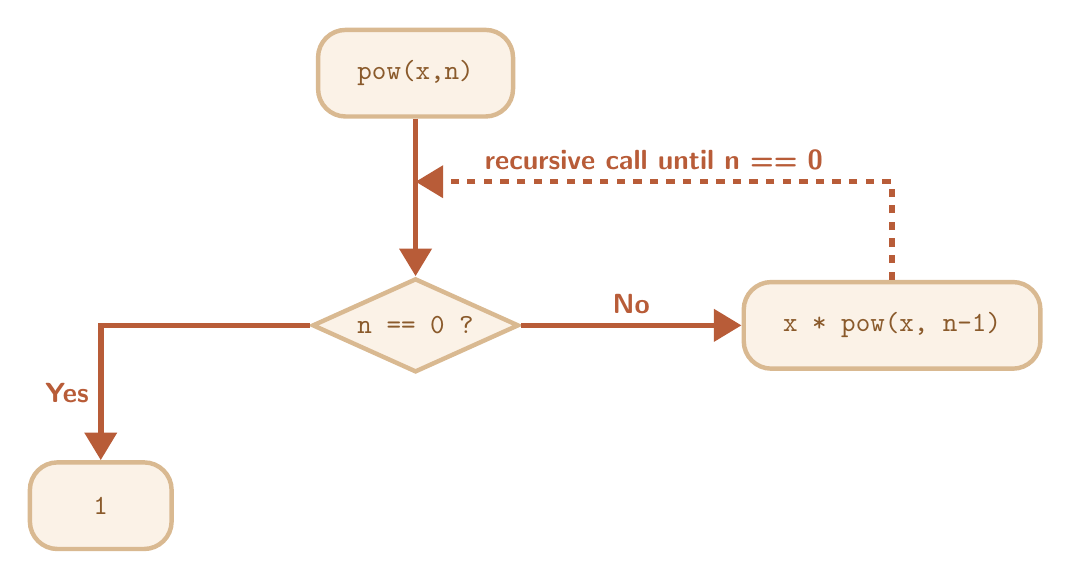
\begin{tikzpicture}[
    font=\ttfamily,
    box/.style={draw=tanline, line width=1.6pt, fill=cream, rounded corners=3.5mm,
                minimum height=11mm, minimum width=18mm, inner xsep=5mm, text=codebrown},
    decision/.style={draw=tanline, line width=1.6pt, fill=cream, diamond,
                     aspect=2.2, inner sep=3pt, text=codebrown},
    flow/.style={-{Triangle[length=3.5mm,width=4mm]}, line width=2pt, draw=rust},
    ret/.style={flow, dashed},
    lab/.style={font=\sffamily\bfseries, text=rust}
]

% nodes
\node[box] (start) {pow(x,n)};
\node[decision, below=20mm of start] (test) {n == 0 ?};
\node[box, right=28mm of test] (recurse) {x * pow(x, n-1)};
\node[box, below left=14mm and 24mm of test] (base) {1};

% flow: entry, then branch on the base-case test
\draw[flow] (start) -- (test);
\draw[flow] (test) -- node[lab, above]{No} (recurse);
\draw[flow] (test.west) -| node[lab, pos=0.75, left]{Yes} (base.north);

% recursive call loops back to the entry arrow
\coordinate (mid) at ($(start.south)!0.4!(test.north)$);
\draw[ret] (recurse.north) |- node[lab, pos=0.75, above]{recursive call until n == 0} (mid);

\end{tikzpicture}
\end{document}
